\documentclass[11pt, letterpaper]{article}

\usepackage[english]{babel} % Sets the language and regional settings for English documents
\usepackage[utf8]{inputenc} % Allows the use of UTF-8 characters in the document
\usepackage[T1]{fontenc} % Specifies t\subsubsection*{Forma canónica reducida}
\usepackage[margin=2cm]{geometry} % Sets the page margins
\usepackage{makeidx} % Enables the creation of indexes
% \usepackage{natbib} % Provides flexible bibliography support
\usepackage{url} % Allows the use of URLs
\usepackage{enumitem} % Customizes the appearance of lists
\usepackage{listings} % Provides syntax highlighting for code listings
\usepackage[dvipsnames]{xcolor} % Allows the use of colors
\usepackage{parskip} % Modifies paragraph spacing
\usepackage{graphicx} % Enables the inclusion of graphics
\usepackage{tikz} % Allows the creation of graphics and diagrams
\usepackage{float}
\usepackage{hyperref} % Enables the creation of hyperlinks
\usepackage{amsmath} % Provides additional math environments and commands
\usepackage{amssymb} % Provides additional math symbols like \ltimes
\usepackage{circuitikz} % Allows the creation of electrical circuits
\usepackage{adjustbox} % Adjusts the size of the circuit diagrams
\usepackage{tcolorbox}
\usepackage{diagbox} % Allows the use of diagonal boxes in table cells
\usepackage{colortbl} % Allows coloring of table cells
\usepackage{fancyhdr} % Allows custom headers and footers
\hypersetup{
    colorlinks=true,
    linkcolor=blue,
    urlcolor=blue
}
\usepackage{breakurl} % permite que los links se rompan en varias líneas
\usepackage{helvet}
\renewcommand{\familydefault}{\sfdefault}

% Configuración adicional para breaks en URLs
\def\UrlBreaks{\do\/\do-\do_\do.\do=\do?\do\&}
\expandafter\def\expandafter\UrlBreaks\expandafter{\UrlBreaks\do\a\do\b\do\c\do\d\do\e\do\f\do\g\do\h\do\i\do\j\do\k\do\l\do\m\do\n\do\o\do\p\do\q\do\r\do\s\do\t\do\u\do\v\do\w\do\x\do\y\do\z}

%Uncomment the following lines to use a sans-serif font
%\usepackage{helvet}
%\renewcommand{\familydefault}{\sfdefault}

\definecolor{mygray}{gray}{0.9}

\usetikzlibrary{shapes.geometric, positioning, decorations.pathreplacing}

\lstset{
	language=SQL,
	basicstyle=\ttfamily\small,
	keywordstyle=\color{blue},
	commentstyle=\color[rgb]{0,0.5,0},
	stringstyle=\color{red},
	numbers=left,
	numberstyle=\tiny\color{gray},
	stepnumber=1,
	numbersep=10pt,
	backgroundcolor=\color{white},
	showspaces=false,
	showstringspaces=false,
	breaklines=true,
	frame=single,
	tabsize=2, captionpos=b, lineskip=-1pt,
	extendedchars=true,
	literate={á}{{\'a}}1 {é}{{\'e}}1 {í}{{\'i}}1 {ó}{{\'o}}1 {ú}{{\'u}}1 {Á}{{\'A}}1 {É}{{\'E}}1 {Í}{{\'I}}1 {Ó}{{\'O}}1 {Ú}{{\'U}}1 {ñ}{{\~n}}1 {Ñ}{{\~N}}1 {¿}{{\textquestiondown}}1 {¡}{{\textexclamdown}}1
}

% VHDL language configuration
\lstdefinelanguage{VHDL}{
	morekeywords={entity, architecture, signal, port, in, out, inout, begin, end, process, if, then, else, elsif, case, when, others, for, while, loop, wait, library, use, std_logic, std_logic_vector, integer, boolean, rising_edge, falling_edge, component, generic, map, downto, to, and, or, not, xor, nand, nor, xnor},
	morecomment=[l]{--},
	morestring=[b]",
	sensitive=false,
	alsoletter={_}
}

% VHDL listings style
\lstdefinestyle{vhdl}{
	language=VHDL,
	basicstyle=\ttfamily\small,
	keywordstyle=\color{blue}\bfseries,
	commentstyle=\color[rgb]{0,0.6,0}\itshape,
	stringstyle=\color{red},
	numbers=left,
	numberstyle=\tiny\color{gray},
	stepnumber=1,
	numbersep=10pt,
	backgroundcolor=\color{white},
	showspaces=false,
	showstringspaces=false,
	breaklines=true,
	frame=single,
	tabsize=2,
	captionpos=b,
	lineskip=-1pt,
	extendedchars=true
}

\lstdefinestyle{cstyle}{
	language=C,
	basicstyle=\ttfamily\small,
	keywordstyle=\color{blue}\bfseries,
	commentstyle=\color[rgb]{0,0.5,0}\itshape,
	stringstyle=\color{red},
	directivestyle=\color{purple},
	numbers=left,
	numberstyle=\tiny\color{gray},
	stepnumber=1,
	numbersep=10pt,
	backgroundcolor=\color{white},
	showspaces=false,
	showstringspaces=false,
	breaklines=true,
	frame=single,
	tabsize=4,
	captionpos=b,
	lineskip=-1pt,
	extendedchars=true,
	literate={á}{{\'a}}1 {é}{{\'e}}1 {í}{{\'i}}1 {ó}{{\'o}}1 {ú}{{\'u}}1 {Á}{{\'A}}1 {É}{{\'E}}1 {Í}{{\'I}}1 {Ó}{{\'O}}1 {Ú}{{\'U}}1 {ñ}{{\~n}}1 {Ñ}{{\~N}}1 {¿}{{\textquestiondown}}1 {¡}{{\textexclamdown}}1
}



\graphicspath{ {./img/} } % Sets the path for the graphics

\newlist{biblio}{enumerate}{1}
\setlist[biblio,1]{label=[\arabic*]}

\makeindex

% \tiny
% \scriptsize
% \footnotesize
% \small
% \normalsize (default size)
% \large
% \Large
% \LARGE
% \huge
% \Huge



% Configure header
\setlength{\headheight}{1pt} % Adjust header height for two-line header
\pagestyle{fancy}
\fancyhf{} % Clear all header and footer fields
\lhead{\textbf{Nombre:} Ugartechea González Luis Antonio -- 320223822 \\ \textbf{Asignatura:} Lab. Fundamentso de Sistemas Embebidos, \textbf{Grupo:} 3}
\renewcommand{\headrulewidth}{0.4pt}

\begin{document}

% \begin{titlepage}

	\begin{tikzpicture}[remember picture,overlay]
		\node[anchor=north west, inner sep=30] at (current page.north west) {
			
\includegraphics[width=4cm]{escudoUNAM_color.png}
		};
		% \node[anchor=north west, inner sep=30] at (current page.north west) {
		% 	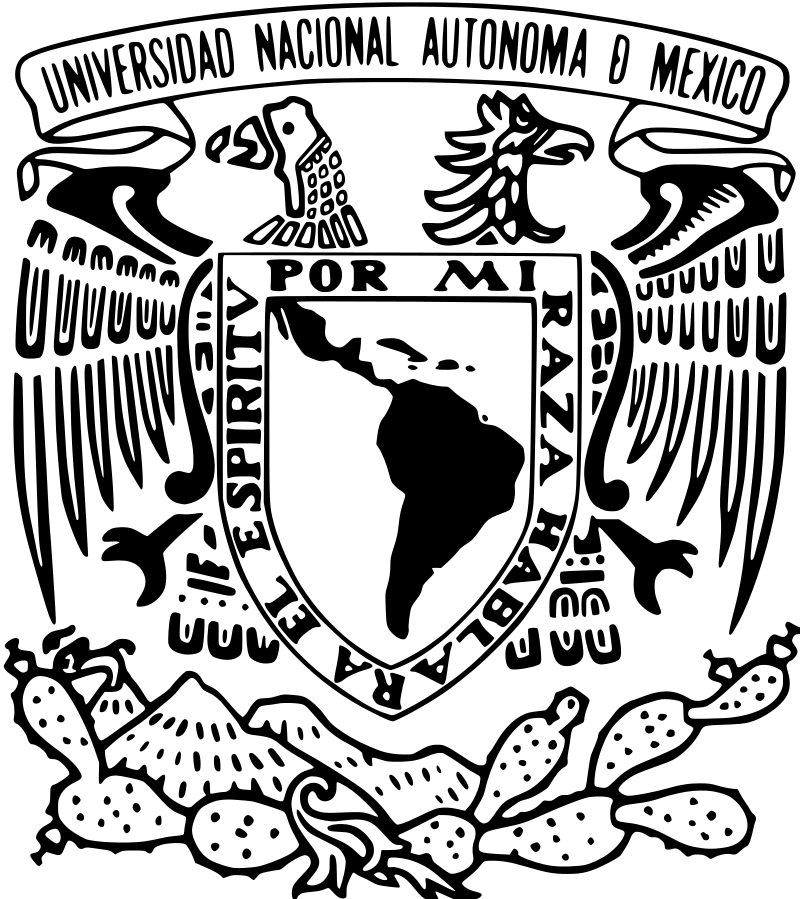
\includegraphics[width=4cm]{escudoUNAM_negro.png}
		% };

		\node[anchor=north east, inner sep=30] at (current page.north east) {
			
\includegraphics[width=4cm]{escudoFI_color.png}
		};
		% \node[anchor=north east, inner sep=30] at (current page.north east) {
		% 	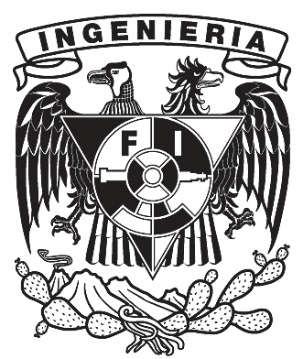
\includegraphics[width=4cm]{escudoFI_negro.png}
		% };
	\end{tikzpicture}

	\begin{center}
		\vspace*{3cm}

		\Huge
		\textbf{Práctica 1 - Lenguaje C para un Sistema Embebido}\\

		\vspace{2.5cm}

		\Huge
		\textbf{Facultad de Ingenieria}\\
		Lab. Fundamentos de Sistemas Embebidos\\
		\textbf{Dr. Eduardo Fragoso Navarro} \\
		2027-1\\

		\vspace{2.5cm}

		%grupo de la materia
		\textbf{Grupo:} 3\\

		\vspace{2.5cm}

		\Huge
		Ugartechea González Luis Antonio\\
		320223822\\
		%fecha de entrega
		\textbf{Fecha de entrega:} 25 de agosto del 2026\\
		\vspace{2.5cm}
	\end{center}
\end{titlepage}

\subsubsection*{Ejercicio 2}

\begin{minipage}{0.45\textwidth}
\begin{adjustbox}{height=0.13\paperheight, width=1\textwidth}
\begin{lstlisting}[style=cstyle, label={lst:ejercicio_2}]
// 4. Una línea diagonal
ssd1306_line(10, 50, 110, 10);
ssd1306_flush();
vTaskDelay(pdMS_TO_TICKS(500));
// 5. Un rectángulo hueco
ssd1306_rect(12, 12, 35, 15);
ssd1306_flush();
vTaskDelay(pdMS_TO_TICKS(500));
// 6. Un rectángulo relleno (usando ssd1306_box)
ssd1306_box(95, 20, 15, 35);
ssd1306_flush();
vTaskDelay(pdMS_TO_TICKS(500));
// 7. Un círculo hueco
ssd1306_circle(64, 32, 15);
ssd1306_flush();
vTaskDelay(pdMS_TO_TICKS(500));
// 8. Un círculo relleno (usando ssd1306_disc)
ssd1306_disc(30, 45, 15);
ssd1306_flush();
vTaskDelay(pdMS_TO_TICKS(500));
// 9. Marco alrededor de todo
ssd1306_rect(0, 0, 128, 64);
ssd1306_flush();
vTaskDelay(pdMS_TO_TICKS(500));
\end{lstlisting}
\end{adjustbox}
\end{minipage}
\hfill
\begin{minipage}{0.6\textwidth}
\begin{figure}[H]
    \centering
    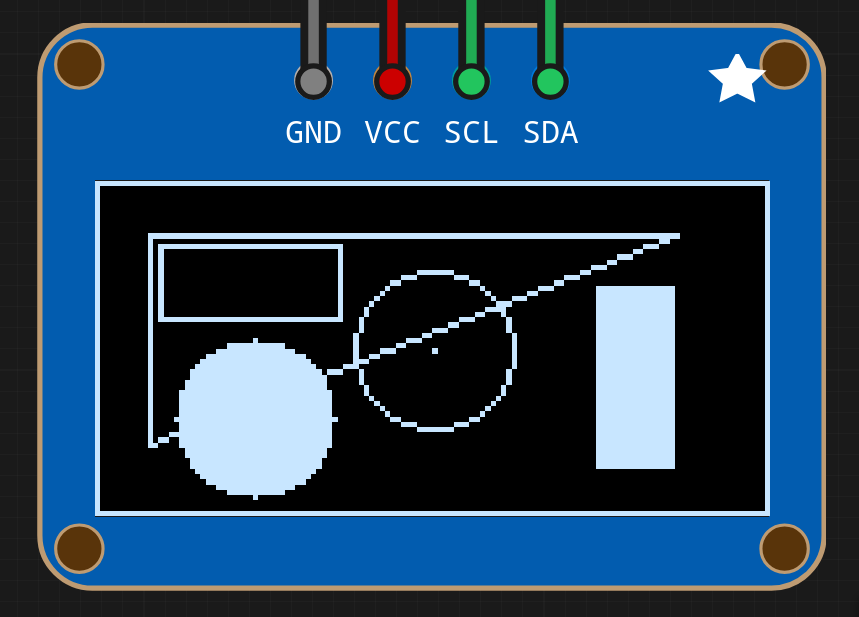
\includegraphics[width=0.9\textwidth]{e2.png}
    \caption{Secuencia completa con todas las figuras.}
    \label{fig:ejercicio_2}
\end{figure}
\end{minipage}


\subsubsection*{Ejercicio 3}

\begin{minipage}{0.45\textwidth}
\begin{adjustbox}{height=0.15\paperheight, width=\textwidth}
\begin{lstlisting}[style=cstyle, label={lst:ejercicio_3}]
#include <math.h>
#ifndef M_PI
#define M_PI 3.14159265358979323846
#endif
void app_main(void) {
    ssd1306_init(5, 6);
    float angulo = 0.0;
    int centro_x = 64;
    int centro_y = 32;
    int radio = 31;
    while(1)
    {
        ssd1306_clear();
        int fin_x = centro_x + (int)(radio * cos(angulo));
        int fin_y = centro_y + (int)(radio * sin(angulo));
        ssd1306_line(centro_x, centro_y, fin_x, fin_y);
        ssd1306_circle(centro_x, centro_y, radio);
        ssd1306_flush();
        angulo += 0.1;
        if (angulo >= 2 * M_PI) {
            angulo -= 2 * M_PI;
        }
        vTaskDelay(pdMS_TO_TICKS(50));
    }
}
\end{lstlisting}
\end{adjustbox}
\end{minipage}
\hfill
\begin{minipage}{0.7\textwidth}
\begin{figure}[H]
    \centering
    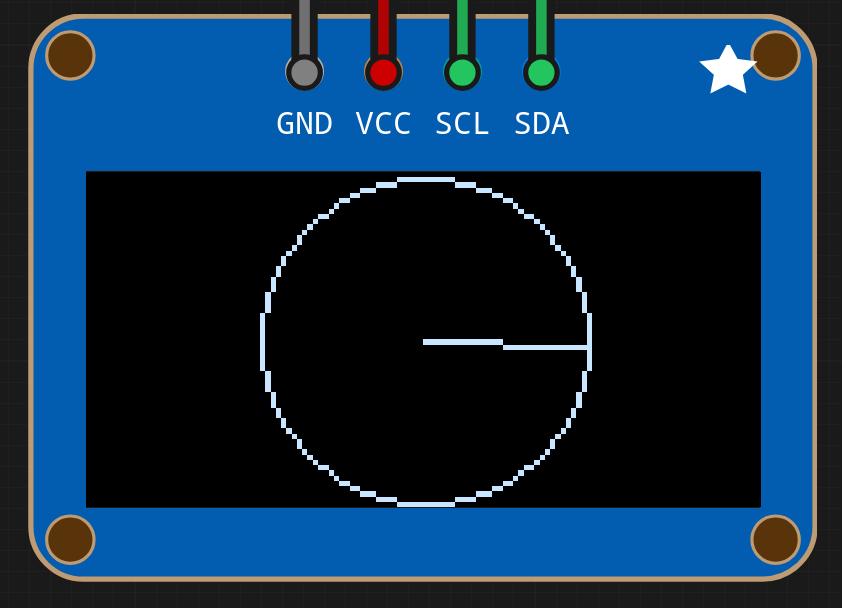
\includegraphics[width=0.4\textwidth]{e3_1.png}
    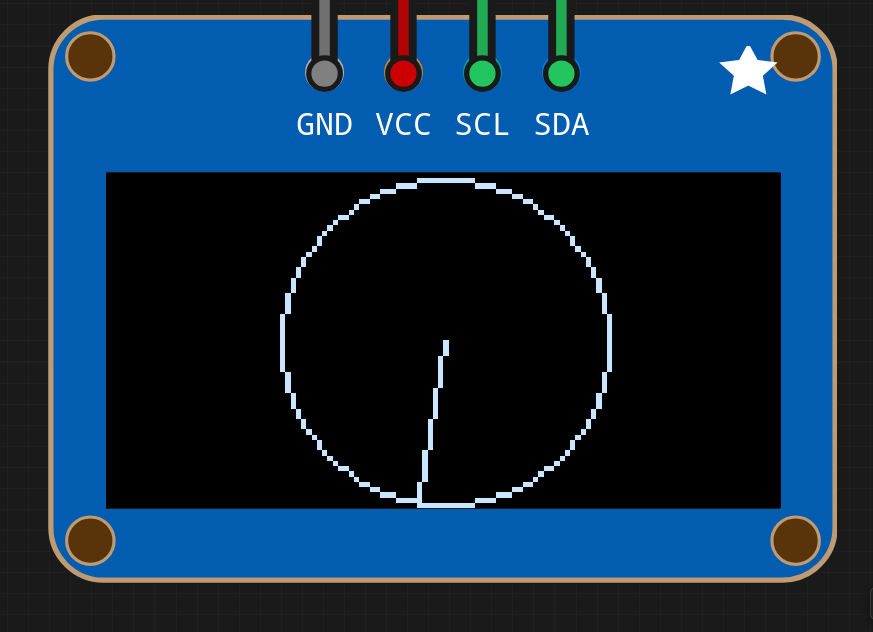
\includegraphics[width=0.4\textwidth]{e3_2.png}
    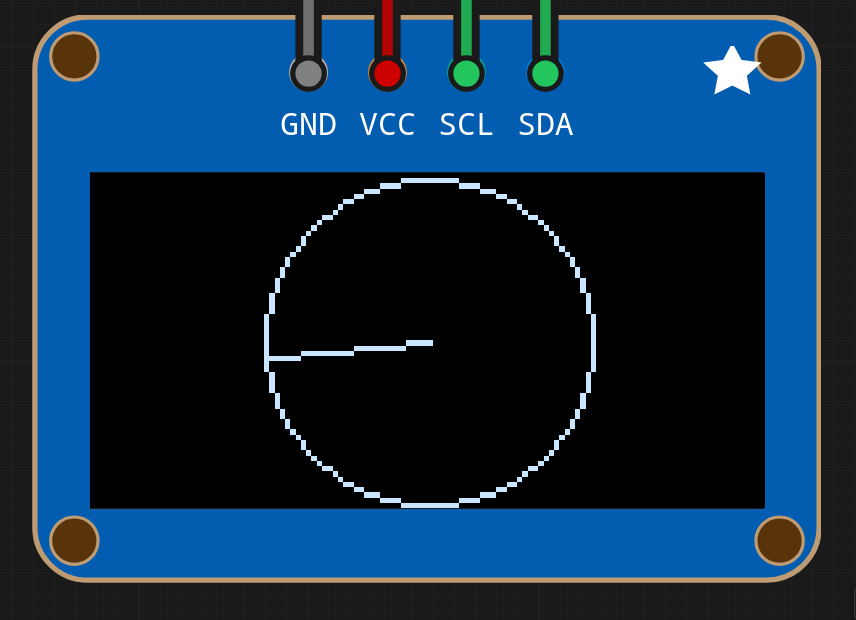
\includegraphics[width=0.4\textwidth]{e3_3.png}
    \caption{Secuencia completa con todas las figuras.}
    \label{fig:ejercicio_3}
\end{figure}
\end{minipage}

\subsubsection*{Conclusión}

Es una buena forma de aprender a utilizar el \texttt{ESP32} debido a que nos ayuda a entender el procedimiento real, a pesar de que el tiempo de simulación con respecto a los retardos puede ser impreciso ya que el simulador depende del procesador de la máquina host de este servicio, en mi caso si docker se sobre carga el tiempo de simulación puede ser afectado. Con respecto al código, la separación de funcionalidad es lo mejor debido a que estamos generalizando el display de figuras sin importar el display que se use, lo único que se cambiaría es el protocolo de comunicación, por otro lado, si se cambia el microcontrolador solo se deben llamar otras librerias para poder hacer el mismo tipo de comunicación I2C dentro de \texttt{ssd1306.c} dependiendo del microcontrolador que se use.

% \section{Bibliografía}

\begin{biblio}
	% for: https://sistemasmultibasededatos.blogspot.com/
	\item Esquivel Martinez H. (2021, Noviembre 28). \textit{SISTEMAS MULTIBASE DE DATOS} [Online]. Disponible en: \newline \textcolor{blue}{\underline{\url{https://sistemasmultibasededatos.blogspot.com/}}}
\end{biblio}

\end{document}
